\chapter{Preliminary Results}
\label{chap:prelim}

\begin{figure}
	\scalebox{0.5}{
	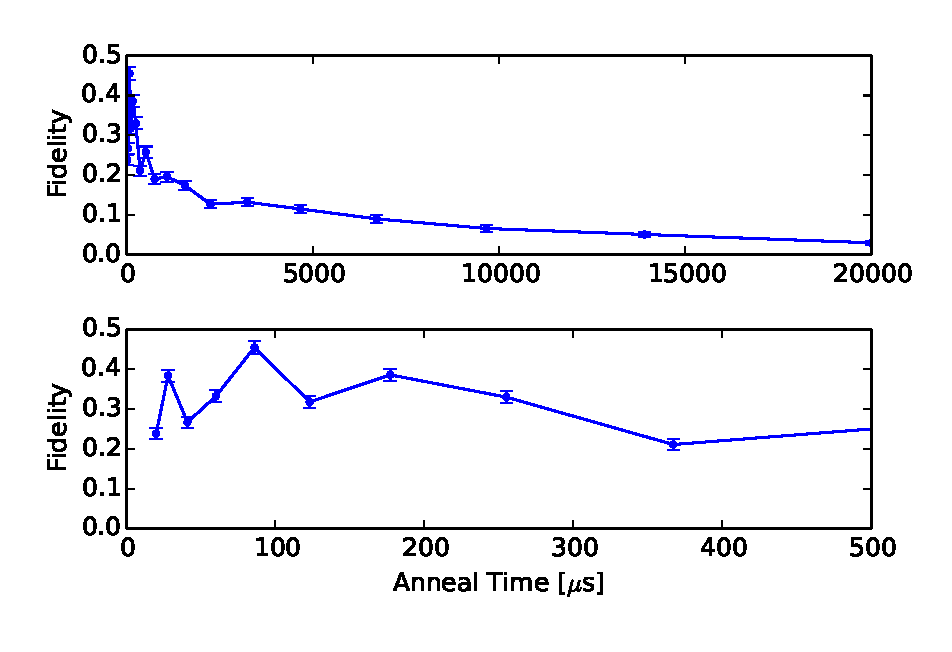
\includegraphics{img/6_018_2_fidelity.eps}
}
\caption[Fidelity vs Time]{Plot of the fidelity as a function of annealing time for the Hamiltonian ``6\_018'' for both the full time range and the first 10 time points.  Both windows show the same data set.  Errors are estimated from $\sigma = \sqrt{np(1-p)}$.  Interesting features include the decrease in fidelity with longer anneal time and that the fidelity is very volatile over the short anneal time periods.}
	\label{fig:fidelity}
\end{figure}

Preliminary results were gathered on a sample quasi-random Hamiltonian called ``6\_018''.  This problem Hamiltonian was built up of clusters of clause sub-Hamiltonians in the same way as a SAT solver Hamiltonian would be, although ``6\_018'' does not encode a actual SAT problem.  This Hamiltonian was simple to generate and allowed us to verify our procedure for analyzing AQC results.
Data was collected in a series of evolutions at annealing times ranging from 20 $\mu$s to 20 ms.  Each evolution consists of choosing an anneal time and programming the problem Hamiltonian onto the hardware, then annealing 1000 times successively and reading out the final states.  We call each of these individual evaluations a \emph{read}, and a whole sequence of reads with the same programmed Hamiltonian a \emph{run}.  Any programming error (see \ref{sec:noise}) in the Hamiltonian should be the same between reads and differ between runs.

The state read out after each read is either the ground state, or some other higher energy (and incorrect) state.  The successes and failures thus follow a binomial distribution; there is some probability $p$ of getting the ground state, and probability $1-p$ of getting a different state.
Our best estimate of the fidelity from a single run is thus the fraction of successes, or $p = \frac{gs}{n}$ for $gs$ reads of the ground state and $n$ total reads.  We can also estimate the error in our estimate of the fidelity, because the variance of a binomial distribution is $\sigma^2 = np(1-p)$.

Figure \ref{fig:fidelity} shows the results of an initial set of runs spanning annealing times from 20 $\mu$s to 20 ms.  There are several features of this data that stand out.  First, contrary to our expectations, the fidelity \emph{decreases} as the anneal time increases.  We would expect that longer anneal times bring us closer to adiabatic evolution and thus remaining in the ground state.  This result suggests to us that adiabaticity (or lack thereof) is not dominating the errors.  Second, there is significant change in the fidelity over very small changes in anneal time for less than $\sim 300$ $\mu$s, well outside what we would statistically expect based on the number of reads conducted.  This suggests that the \texttt{VESUVIUS} machine cannot be naively treated as an adiabatic quantum system.

The two main questions this work seeks to address are thus: \emph{Why does the fidelity vary so greatly for short anneal times, and why does the fidelity decrease for longer anneal times?}

\begin{figure}
	\scalebox{0.35}{
		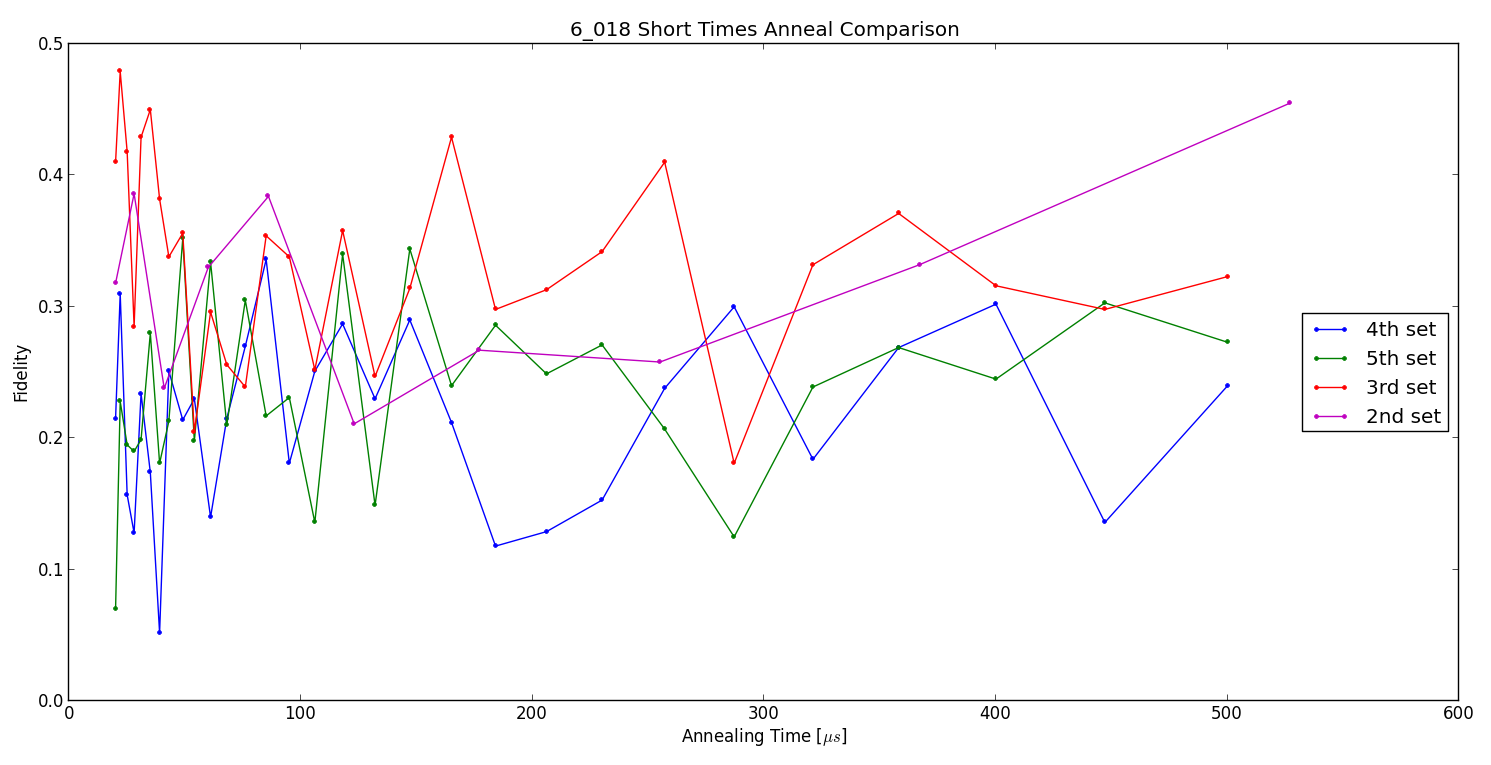
\includegraphics[bb= 0 0 745 382]{img/6_018_comparison.png}
	}
	\caption[Short Time Fidelities]{The fidelity as a function of time for the Hamiltonian ``6\_018'' for several different machine runs.  Each data point consist of 1000 machine reads.  Notice the spread between machine runs is outside of the error bars.}
	\label{fig:short_fidelity}
\end{figure}

\section{Short-time Evolution}
Figure \ref{fig:short_fidelity} shows the results of four different sets of runs of the Hamiltonian ``6\_018''.  As can be seen, the estimated fidelities lie well apart from each other, and outside their respective estimated errors.  This would seem to indicate that programming errors are a significant factor in the final fidelity: for the same anneal time on the same Hamiltonian, different runs of ``6\_018'' have fidelities ranging from 0.07 to 0.41.


\section{Long-time Evolution}
For a purely quantum system the fidelity should increase in the limit of increasing annealing time.  What we see instead in the actual data is that the fidelity appears to approach zero as the annealing time increases.  The physical computer is not an ideal quantum system, so to model it correctly we need to account for noise and decoherence sources.

We should fit this decreasing fidelity, or perhaps the population histogram, to some sort of model of thermal noise.  Then we could determine the energy leakage, maybe.




\begin{figure}
	\scalebox{0.75}{
		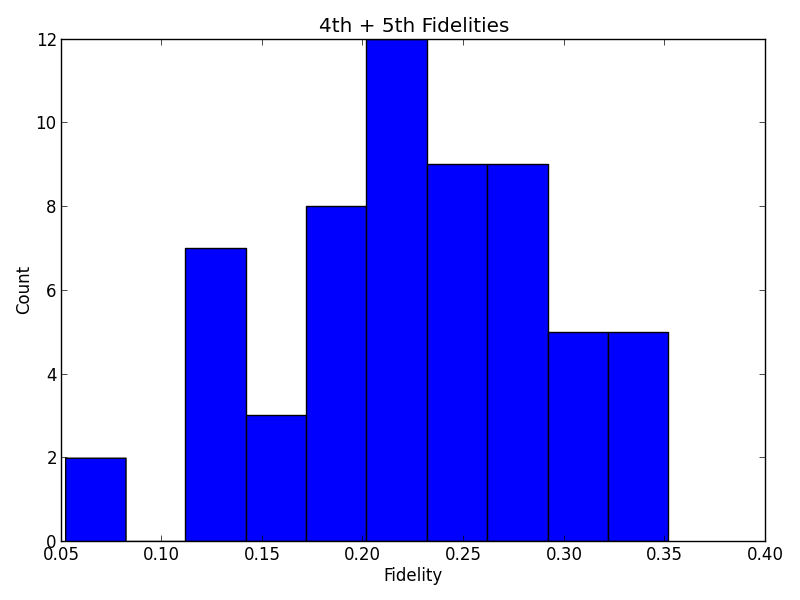
\includegraphics[bb= 0 0 800 600]{img/4_5_hist.png}
	}
	\caption[Short Time Fidelity Histogram]{Histogram of the fidelities found for all annealing times  $< 500 \mu$s.  Notice the gaussian like structure.}
	\label{fig:fid_hist}
\end{figure}

\begin{figure}
	%\scalebox{0.75}{
	%	\includegraphics[]{}
	%}
	\caption[Simulation of Schr\"odinger's Equation]{Numerical integration of Schr\"odinger's Equation for the Hamiltonian ``k44'' showing the fidelity increasing to a plateau as the annealing time increases.}
	\label{fig:simulated_anneal}
\end{figure}

\begin{figure}
	%\scalebox{0.75}{
	%	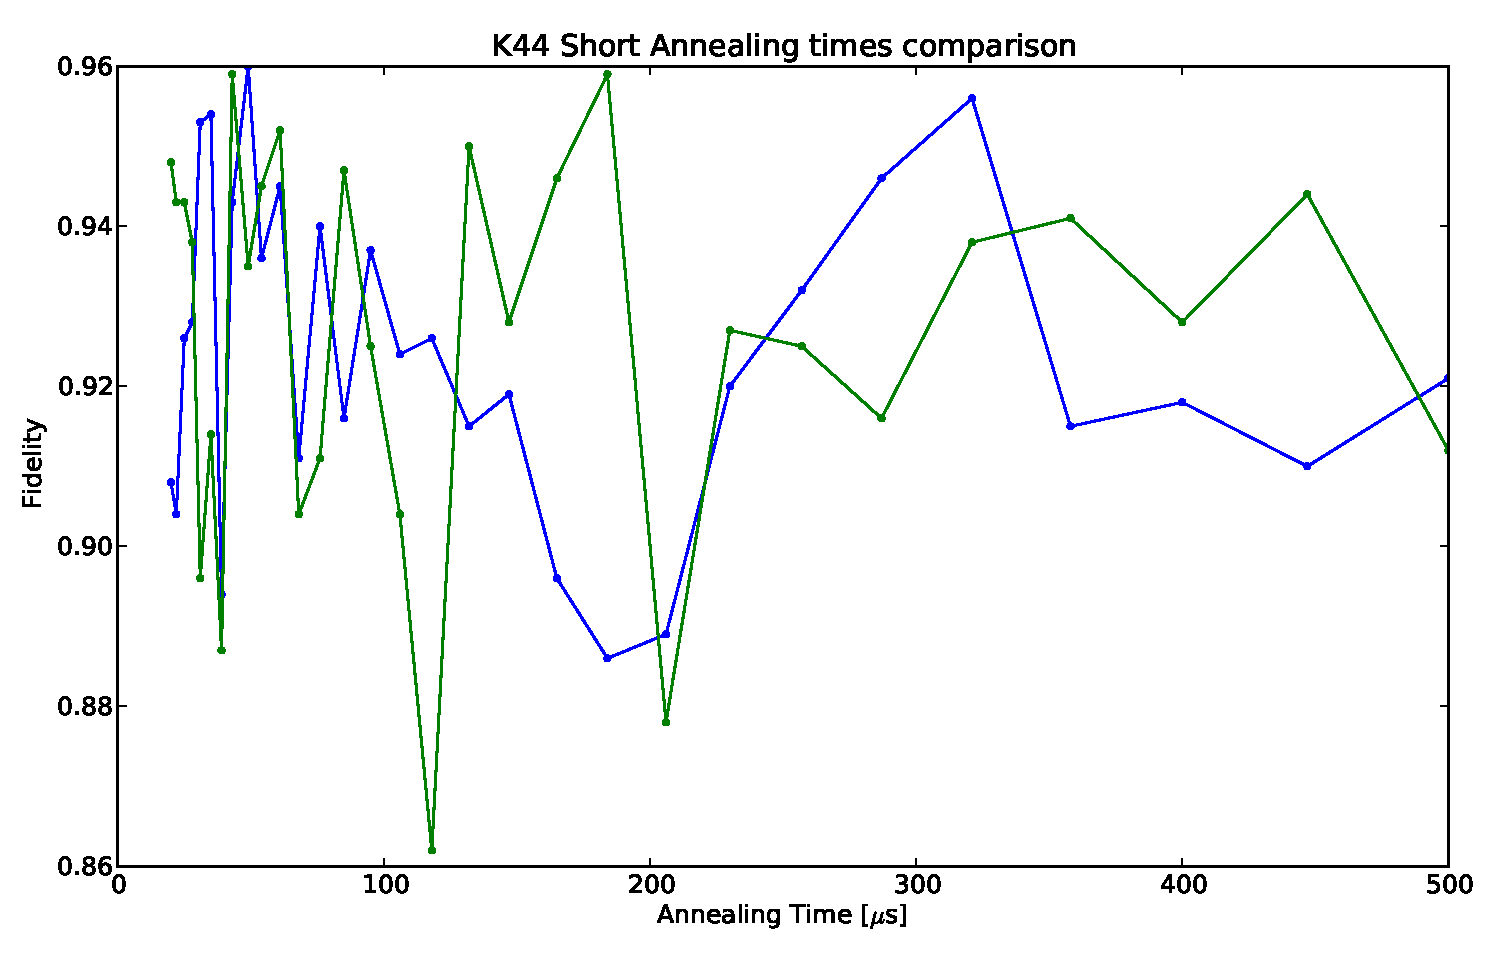
\includegraphics{img/k44_comparison.pdf}
	%}
	\caption[Long Time Anneal]{Machine data from Hamiltonian ``k44'' with 100 runs of 1000 reads showing the Hamiltonian noise at short times and the fidelity drop at long anneal times.}
	\label{fig:k44_long}
\end{figure}
